\chapter{Series Solutions of Second-Order Linear Equations}

\section{Review of Power Series}

Before we do a \textit{deep dive} into how to use power series to solve differential equations,
let us first recall what power series are. Firstly, recall what power series look like.

\[ \sum_{n=0}^\infty a_n {(x - x_0)}^n \]

Additionallly, some useful concepts relating to power series are the following.

\begin{enumerate}
    \item Power series $\sum_{n=0}^m a_n {(x - x_0)}^n$ is said to converge at given point $x$ if 
        \[ \lim_{m \to \infty} \sum_{n=0}^m a_n {(x - x_0)}^n \]
        exists for said $x$. The series clearly converges for when $x = x_0$. However, it may
        converge for all $x$ or only some, depending on the actual values.
    \item Power series $\sum_{n=0}^m a_n {(x - x_0)}^n$ \textit{converges absolutely} at point $x$
        associated power series of its absolutes
        \[ \sum_{n=0}^\infty |a_n{(x - x_0)}|^n = \sum_{n=0}^\infty |a_n||x - x_0|^n \]
        converges. If a power series converges absolutely, the it also converges. The converse,
        however, is not always true.
    \item \textit{Ratio Test} $-$ For some fixed value of $x$ and $a_n \neq 0$,
        \[ \lim_{n\to\infty} \left|\frac{a_{n+1}{(x-x_0)}^{n+1}}{a_n{(x - x_0)}^n}\right|
        = |x-x_0|\lim_{n\to\infty} \left|\frac{a_{n+1}}{a_n}\right| = |x-x_0|L \]
        then the power series
        \begin{itemize}
            \item converges absolutely if $|x - x_0|L < 1$
            \item diverges if $|x - x_0|L > 1$
            \item is inconclusive if $|x - x_0|L = 1$
        \end{itemize}
    \item If given power series $\sum_{n=0}^\infty a_n{(x - x_0)}^n$ converges at $x = x_1$, it converges
        absolutely for $|x - x_0| < |x_1 - x_0|$. If it diverges at $x = x_1$, it diverges for
        $|x - x_0| > |x_1 - x_0|$.
    \item For a typical power series, there exists a positive number $\rho$, called the 
        \textbf{radius of convergence}, such that $\sum_{n=0}^\infty a_n{(x - x_0)}^n$ always converges
        absolutely for all $|x - x_0| < \rho$ and diverges for all $|x-x_0| > \rho$. This interval where
        the series converges is called the \textbf{interval of convergence}. At $|x-x_0| = \rho$, 
        the series may converge or diverge.

        \begin{center}
            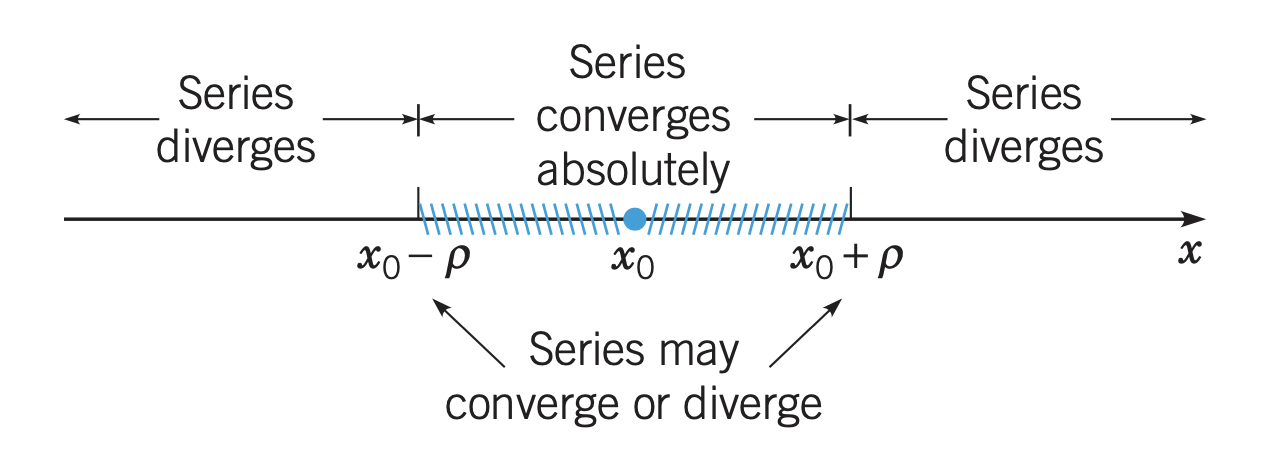
\includegraphics[scale=0.5]{05/interval-of-convergence.png}
        \end{center}
\end{enumerate}

Now, suppose that $\sum_{n=0}^\infty a_n{(x-x_0)}^n$ and $\sum_{n=0}^\infty b_n{(x-x_0)}^n$ converges 
to $f(x)$ and $g(x)$, respectively, for $|x-x_0| < \rho$ and $\rho > 0$.

\begin{enumerate}
    \setcounter{enumi}{5}
    \item The two series can be added or subtracted termwise, meaning
        \[ f(x) \pm g(x) = \sum_{n=0}^\infty (a_n \pm b_n){(x-x_0)}^n \]
        and it will converge at least for $|x - x_0| < \rho$.
    \item The two series can be multiplied by
        \[ f(x)g(x) = \sum_{n = 0}^\infty c_n{(x - x_0)}^n \] 
        where $c_n = a_0 b_n + a_1 b_{n-2} + \cdots + a_n b_0$ and it will converge at least for
        $|x - x_0| < \rho$.

        Additionally, given that $b_0 \neq 0$ and $g(x_0) \neq 0$, series for $f(x)$ is divisible by series for $g(x)$,
        and \[ \frac{f(x)}{g(x)} = \sum_{n=0}^\infty d_n{(x - x_0)}^n \]
        $d_n$ can be most easily obtained by solving the following relation
        \begin{align*}
            \sum_{n=0}^\infty a_n{(x-x_0)}^n
                &= \left(\sum_{n=0}^\infty d_n{(x-x_0)}^n\right) \left(\sum_{n=0}^\infty d_n{(x-x_0)}^n\right)\\
                &= \sum_{n=0}^\infty\left(\sum_{k=0} d_k b_{n-k}\right){(x-x_0)}^n
        \end{align*}

        In the case of division, the radius of convergence of resulting series may be less than $\rho$.
    \item Function $f(x)$ is continuous and has derivatives of all orders for $|x-x_0| < \rho$.
        Additionally, derivatives of all orders can be computed by differentiating the series termwise
        and each series (in the derivatives) converges absolutely for $|x-x_0| < \rho$.
    \item Value of $a_n$ is given by \[ a_n = \frac{f^{(n)}(x_0)}{n!} \]
        This is essentially the Taylor series for the function $f$ about $x = x_0$.
    \item If both series are equivalent for each $x$ in some open interval with center $x_0$,
        then $a_n = b_n \forall\ n = 0, 1, 2, \cdots$. If $\sum_{n=0}^\infty a_n{(x - x_0)}^n = 0$ for 
        each such $x$, then $a_0 = a_1 = \cdots = a_n = \cdots = 0$.
\end{enumerate}

A function $f$ with Taylor Series Expansion about $x = x_0$
\[ f(x) = \sum_{n=0}^\infty \frac{f^{(n)}(x_0)}{n!}{(x - x_0)}^n \]
with radius of convergence $\rho > 0$ is said to be \textbf{analytic} at $x = x_0$.
Given that $f$ is analytic at $x_0$, then $f \pm g$, $f \cdot g$, and $f / g$ (for $g \neq 0$) are
also analytic at $x = x_0$.

\subsection{Shift of Index Summation}

Index of summation in an infinite series is a dummy variable, implying that whatever letter we use to 
represent it, it will not matter. For instance,
\[ \sum_{n = 0} \frac{2^n x^n}{n!} \equiv \sum_{j=0}^\infty \frac{2^j x^j}{j!} \]
This means that we can shift the summation indices to compute series solutions.

\begin{example}
We want to write $\sum_{n=2}^\infty a_n x^n$ as a series that starts from $n=0$ instead of $n=2$.

A way to do this is to let $m = n-2$, then $n = m+2$. Thus, $n=2$ corresponds to $m = 0$. Hence,
\[ \sum_{n=2}^\infty a_n x^n = \sum_{m=0}^\infty a_{m+2} x^{m+2} \]

What we have done here is essentially shifting the index upward by two while making the initial value
of $n = 0$.
\end{example}